\documentclass[10pt]{article}

\usepackage{mathtools, amssymb, bm}
\usepackage{microtype}
\usepackage[utf8]{inputenc}
\usepackage[margin = 0.75in]{geometry}
\usepackage{booktabs}
\usepackage{graphicx}
\usepackage{xcolor}
\usepackage{tikzsymbols}
\usepackage[hidelinks]{hyperref}
\usepackage{titlesec}

\usepackage{wrapfig}

% \titleformat{\section}{\normalsize\bfseries}{\thesection}{1em}{}
\titleformat{\section}{\large\bfseries}{\thesection}{1em}{}
\setcounter{secnumdepth}{0}

\definecolor{colabcol}{HTML}{960018}
\newcommand{\mycolab}[1]{\textcolor{colabcol}{\textsl{Collaborators:}} #1 \\ }
\newcommand{\mycolaba}[1]{\textcolor{colabcol}{\textsl{Collaborators:}} #1}

\title{
    {\Large Homework 2}
}
\author{
    {\normalsize Aiden Kenny}\\
    {\normalsize STAT GR5205: Linear Regression Models}\\
    {\normalsize Columbia University}
}
\date{\normalsize Octover 23, 2020}

\begin{document}

\maketitle

%' ============================================================================================================================================================
\section{Question 1} \noindent
We are considering the linear regression model 
\begin{align*}
    Y = \beta_0 + \beta_1 X + \epsilon,
\end{align*}
where \(\hat{Y}\) is the estimated service time for a call, \(X\) is the number of copiers being serviced,
and \(\epsilon \sim \mathrm{N}(0,\sigma^2)\). 
The least-squares estimator model is given by 
\begin{align}
    \hat{Y} = -0.5802 + 15.0352X \label{copier-lm}
\end{align}
% The data and the estimated model are both plotted in Figure \ref{copier-plot}. Visually, it is clear that
% least-squares model fits the data extremely well.
Throughout this question, we will be using a variety of base R functions to easily obtain the desired measurements. 
% \begin{figure}[h]
%     \centering
%     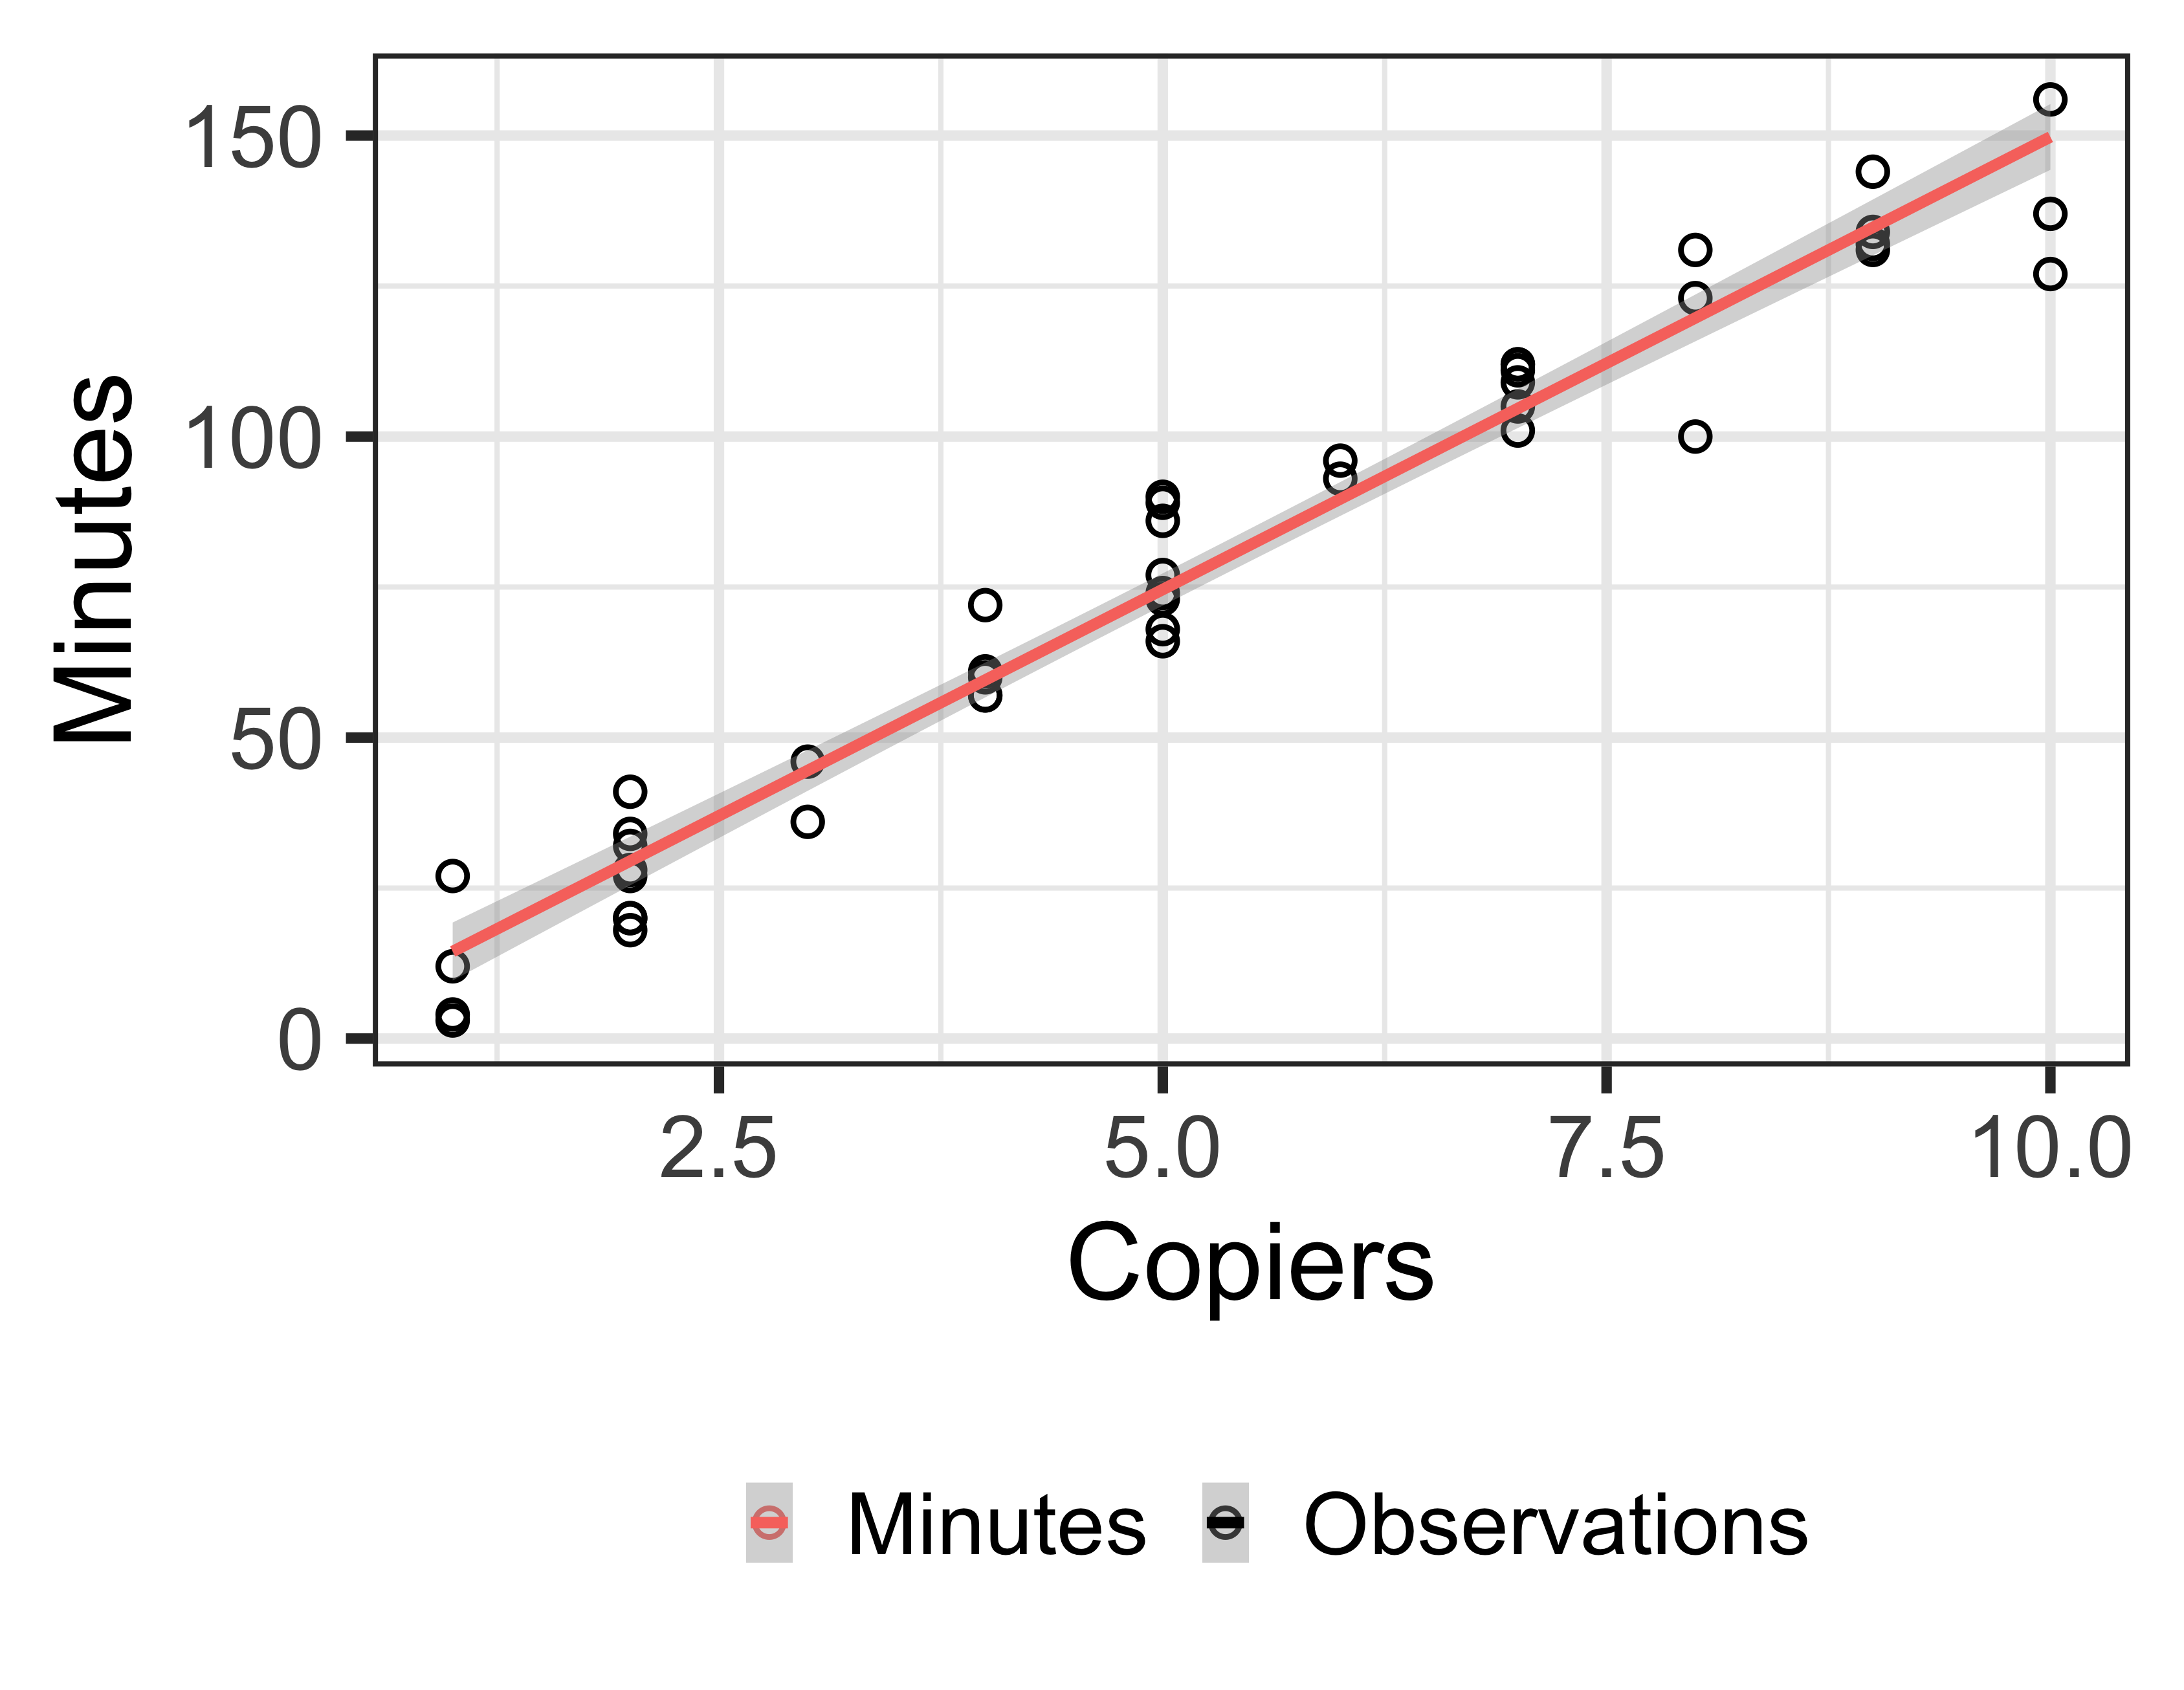
\includegraphics[width = 0.35\textwidth]{img/copier-linear.png}
%     \caption{A plot of model \ref{copier-lm}.}
%     \label{copier-plot}
% \end{figure}
% \begin{wrapfigure}{R}{0.35\textwidth}
%     \centering
%     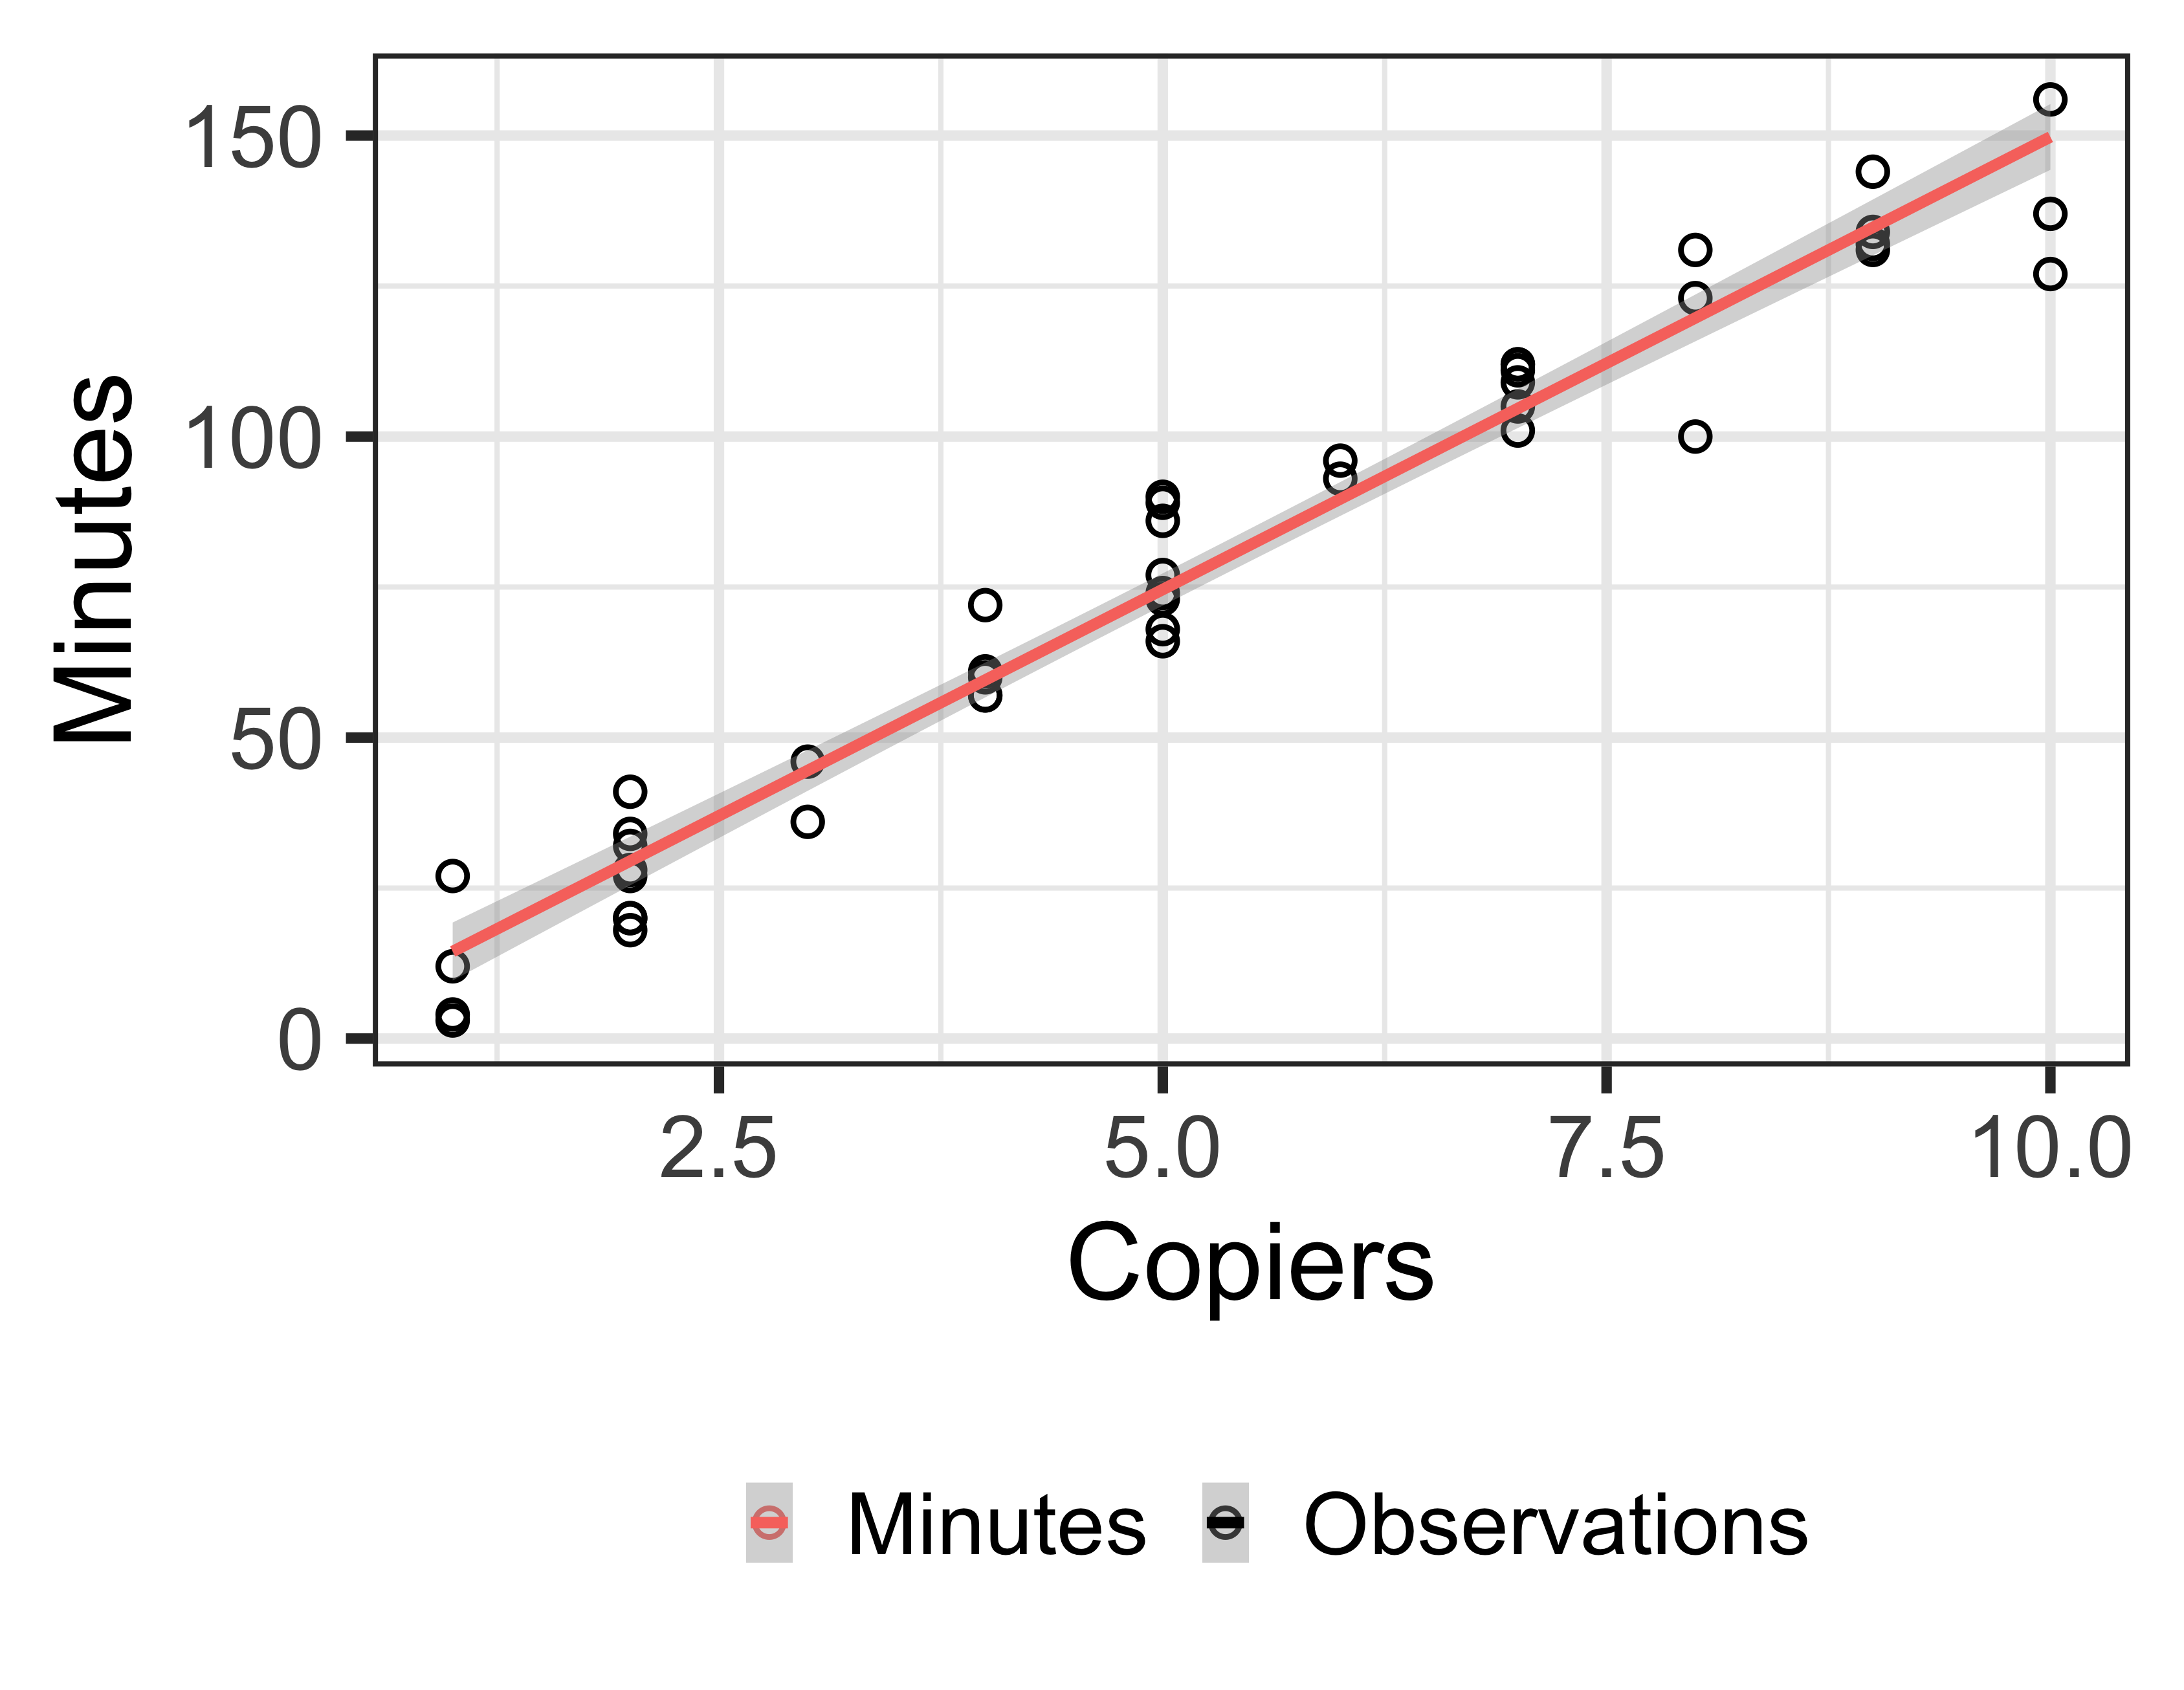
\includegraphics[width = 0.35\textwidth]{img/copier-linear.png}
%     \caption{A plot of model \ref{copier-lm}.}
%     \label{copier-plot}
% \end{wrapfigure}
\begin{itemize}
    \item[(a)] The \(95\%{}\) confidence interval for the mean service time when there are six copiers is given by 
    \begin{align*}
        \mathrm{E}[Y] \in \Big(86.8152, 92.44746 \Big).
    \end{align*}
    Intuitively, this means that there are six copiers being serviced, we are \(95\%{}\) sure that the average service time for 
    \textsl{all} service times falls within this range. 
    \item[(b)] The \(95\%{}\) prediction interval for the next service time when there are six copiers is 
    \begin{align*}
        \widehat{Y} \in \Big( 71.43628, 107.8264 \Big).
    \end{align*}
    As expected, we notice that the prediction interval is significantly wider than the confidence interval. 
    \item[(c)] 
    \item[(d)] The ANOVA table has been printed in Table \ref{copier-anova}.
    \begin{table}
        \centering
        \def\arraystretch{1.25}
        \begin{tabular}[ht]{lccccc} \toprule
            Source of Variation & \(\mathrm{df}\) & Sum of Squares & Mean Square & \(f\) & \(\mathrm{Pr}(> f)\) \\\midrule
            Copiers & \(1\) & \(76960\) & \(76960\) & \(968.66\) & \(< 2.2 \times 10^{-16}\) \\
            Residuals & \(43\) & \(3416\) & \(79\) & -- & -- \\
            Total & \(44\) & \(80376\) & -- & -- & -- \\\bottomrule
        \end{tabular}
        \caption{The ANOVA table for model (\ref{copier-lm}).}
        \label{copier-anova}
    \end{table}
    \item[(e)] To determine if there is any linear relationship between \(X\) and \(Y\), we conduct an \(F\)-test, where 
    \(H_0 : \beta_1 = 0\) against \(H_a : \beta_1 \neq 0\). From Table \ref{copier-anova}, we see that the associated \(p\)-value is 
    well below the significance level \(\alpha = 0.05\), and so we reject \(H_0\). The data seems to indicate that there is in fact a 
    linear relationship between \(X\) and \(Y\).
    \item[(f)] The total variance explained by the model is known as the \(R^2\) value, and is given by
    \begin{align*}
        R^2 = \frac{\mathrm{SSR}}{\mathrm{SST}} = \frac{76960}{80376} \approx 0.9575.
    \end{align*}
    That is, bout \(95.7\%{}\) of \(Y\)'s variation is explained by model (\ref{copier-lm}), quite a significant reduction. 
\end{itemize}

%' ============================================================================================================================================================
\section{Question 2} \noindent


\end{document}